\section{Experimental details}
\label{app:experiments}

This section gives the details of Sections~\ref{sec:analytic}, \ref{sec:rates} and~\ref{sec:numerical}, with
$\delta=0.05$ throughout.

\subsection{Synthetic designs}

Table~\ref{tab:hardern80} and Figure~\ref{fig:recovery} of the main text use the designs of
Table~\ref{tab:harderdesigns}. Each follows \eqref{eq:contam} with a mixture weight $a$ in place of $\alpha$, so that
$\TV(P,Q)=a\,\TV(P_0,Q_0)$ whatever the common component $R$; in the overlap and shift designs $R=N(0,I)$ and
$a=\tfrac14$, and mutually singular $P_0$ and $Q_0$ give $\alpha^\star=a$. The module
\texttt{explore/harder\_sims/designs.py} of the repository of Section~\ref{sec:computationdetails} defines every design,
its core, weight and contaminations, and \texttt{explore/harder\_sims/DESIGN.md} derives each $\alpha^\star$.

\begin{table}[t]
\centering
\scriptsize
\setlength{\tabcolsep}{4pt}
% Generated by tools/derive.py from tables/harder_designs.tex and explore/harder_sims/out/popmmd.csv -- do not edit.
% Generated by jmlr/tools/make_harder_tables.py from results/harder/ (harder synthetic study). Do not edit.
\begin{tabular}{llcccc}
\toprule
design & $P_0$ vs $Q_0$ & $d$ & $n$ & $\alpha^\star$ & $\MMD$ \\
\midrule
RHC-shaped & RHC core, boxes at $\pm$3 SD & $33$ & $100$--$800$ & $0.2$ & $0.201$ \\
overlap, $d=2$ & $N(\pm\mu e_1,I)$ & $2$ & $100$--$800$ & $0.1$ & $0.091$ \\
overlap, $d=2$ & $N(\pm\mu e_1,I)$ & $2$ & $100$--$1600$ & $0.2$ & $0.181$ \\
overlap, $d=10$ & $N(\pm\mu e_1,I)$ & $10$ & $100$--$800$ & $0.1$ & $0.042$ \\
overlap, $d=10$ & $N(\pm\mu e_1,I)$ & $10$ & $100$--$800$ & $0.2$ & $0.103$ \\
dense shift, $d=20$ & $N(\pm\mu\mathbf 1/\sqrt d,I)$ & $20$ & $100$--$800$ & $0.2$ & $0.077$ \\
dense shift, $d=50$ & $N(\pm\mu\mathbf 1/\sqrt d,I)$ & $50$ & $100$--$800$ & $0.2$ & $0.048$ \\
dense shift, $d=100$ & $N(\pm\mu\mathbf 1/\sqrt d,I)$ & $100$ & $100$--$800$ & $0.2$ & $0.038$ \\
sparse shift, $d=50$ & $N(\pm\mu(e_1+e_2)/\sqrt2,I)$ & $50$ & $100$--$800$ & $0.2$ & $0.049$ \\
correlation flip, $d=50$ & $\operatorname{corr}(x_1,x_2)=\pm\rho$ & $50$ & $100$--$800$ & $0.2$ & $\approx0$ \\
small contamination, $d=2$ & $N(\pm2.5e_1,0.25I)$, $a=0.05$ & $2$ & $100$--$1600$ & $0.05$ & $0.050$ \\
mixed types, $m=5n$ & integer and binary coordinate & $5$ & $100$--$400$ & $0.2$ & $0.135$ \\
$t_3$ tails, $d=5$ & scale $0.5$ vs $3$ of $x_1$ & $5$ & $100$--$800$ & $0.2$ & $0.076$ \\
curves, wide bump & $\pm$ bump of width $0.2$ & $50$ & $100$--$800$ & $0.2$ & $0.118$ \\
curves, narrow bump & $\pm$ bump of width $0.05$ & $50$ & $100$--$800$ & $0.2$ & $0.043$ \\
oscillating, $\nu=1$ & $U[0,1]$ vs density $1+\varsigma(\nu x)$ & $1$ & $100$--$800$ & $0.5$ & $0.492$ \\
oscillating, $\nu=4$ & $U[0,1]$ vs density $1+\varsigma(\nu x)$ & $1$ & $100$--$800$ & $0.5$ & $0.069$ \\
oscillating, $\nu=16$ & $U[0,1]$ vs density $1+\varsigma(\nu x)$ & $1$ & $100$--$800$ & $0.5$ & $0.019$ \\
oscillating, $\nu=64$ & $U[0,1]$ vs density $1+\varsigma(\nu x)$ & $1$ & $100$--$800$ & $0.5$ & $\approx0$ \\
\bottomrule
\end{tabular}

\caption{The synthetic designs of Section~\ref{sec:numharder}: $P_0$ against $Q_0$ ($P$ against $Q$ for the oscillating
designs); sizes $n=m$ at which every method that certifies a level was run, doubling ($m=5n$ for mixed types);
$\alpha^\star$, exact (small contamination: $0.05\,(2\Phi(5)-1)$); population MMD at the analytic test's bandwidth, by
Monte Carlo ($\approx0$: estimate of $\MMD^2$ not positive).}
\label{tab:harderdesigns}
\end{table}

All methods see the same $\harderReps$ replicates per design and size. The permutation test and MMDAgg, which uses
$\abAggL$ Gaussian bandwidths, were run up to $n=m=\harderNmax$, and to $1{,}600$ on the narrow bump. The tests of
$H_{0,0}$ that certify a level were continued: every design and method below power $0.8$ at $n=m=\harderNmax$ ($n=400$
for mixed types) was run at $n=m=1600$, $3200$, $6400$ and $\harderNcap$ (from $n=800$, with $m=5n$, for mixed types),
with $\harderExtReps$ new replicates per size, until its power was at least $0.8$ at two consecutive sizes, in
$\harderExtCells$ design and size cells, and the four nulls with $P=Q$ below in $\harderNullExtCells$ cells
($\harderNullExtReplicates$ replicates). The methods of Section~\ref{sec:baselines} see the replicates of the main size,
with the same data, folds and bandwidths. Gradient boosting's drop on the correlation flip at $n=\harderNcap$ is
scikit-learn's default early stopping above $10{,}000$ training points; without it its power is $\harderFlipEsPowOff$
instead of $\harderFlipEsPowOn$ ($\harderFlipEsReps$ replicates).

The analytic test and the permutation test take their Gaussian bandwidth from one pilot draw per design, $1000+1000$
points ($400+2000$ for mixed types), as the median pairwise distance of the pooled pilot. Every analytic number of the
main text and of this section uses $\tau=\min\{\tau^{\mathrm P},\tau^{\mathrm S}\}$, which equals $\tau^{\mathrm P}$ at
every size and level of these runs, so the analytic test is that of Theorem~\ref{thm:plugin};
Section~\ref{sec:kernelfallback} says where another threshold is used. The Laplace ramp cuts its witness
at genuine empirical quantiles (Algorithm~\ref{alg:split}), and the Gaussian ramp, the untrimmed witness and the check
of Section~\ref{sec:excessmc} between order statistics, within one rank of genuine quantiles \eqref{eq:cutrank}. The
classifiers, histogram gradient boosting with default settings and logistic regression with unit $L^2$ penalty, label a
point as from $P$ when its fitted probability exceeds $n_{\mathrm{tr}}/(n_{\mathrm{tr}}+m_{\mathrm{tr}})$, with
$n_{\mathrm{tr}}$ and $m_{\mathrm{tr}}$ the numbers of $X$'s and $Y$'s they are trained on. The simulations test the levels $j\alpha^\star/8$, $j=0,\dots,10$, which use the known
$\alpha^\star$ and serve only to measure recovery; the real data use the grid $0,0.05,\dots,0.95$.

The null boundary of Section~\ref{sec:analytic} is that of a standard Gaussian core in $d=2$ with contaminations
uniform on two disjoint boxes and $\alpha^\star=0.2$. With $\calibReps$ replicates per level at $n=m=300$, no replicate
rejected $H_{0,\alpha}$ at $\alpha\ge\alpha^\star$ (one-sided $95\%$ Clopper--Pearson upper limit $\calibCPUpper$), and at
$\alpha=\alpha^\star$ the threshold $\tau^{\mathrm P}$ is $\stCalibRatioTauP$ times the empirical $1-\delta$ quantile of
$\widehat D_\alpha$.

In the designs, the Laplace ramp rejected the true null $H_{0,\alpha^\star}$ in at most a fraction $\mnBdMax$ of the
replicates of a design (binomial $p=\mnBdMaxP$), its rate under $P=Q$ lies between $\mnNullLoPct$ and $\mnNullHiPct\%$ in every cell, and its
bound exceeded $\alpha^\star$ in at most a fraction $\mnAloGtMax$ of the replicates of any design. The analytic test
rejected in none of its $\mnAnBdCells$ boundary cells and never under $P=Q$. The other methods were checked in the
same way. At the boundary, in the $\harderBoundaryCells$ cells of the eighteen designs other than the RHC-shaped one,
the Gaussian ramp rejected at most $\hvBdWorstRamp$ times in a cell, gradient boosting $\hvBdWorstGbm$ and logistic
regression $\hvBdWorstLogit$. On the RHC-shaped design the three rejected $\dNineRampBdMax$, $\dNineGbmBdMax$ and
$\dNineLogitBdMax$ times. All these counts are below the $\harderFlagK$ rejections at which a binomial test against
$\delta$ at level $0.01$ flags a cell.
Four nulls with $P=Q$, on which every bet has mean exactly $\alpha=0$, use the law $P$ of the dense-shift ($d=100$),
mixed-type, $t_3$ and narrow-bump designs; up to $n=800$ the Gaussian ramp rejected in $\hvNullRamp\%$ of the
replicates, gradient boosting in $\hvNullGbm\%$ and logistic regression in $\hvNullLogit\%$, and up to $n=\harderNcap$
at most $\harderNullExtMaxRamp$, $\harderNullExtMaxGbm$ and $\harderNullExtMaxLogit$ times in a cell of
$\harderExtReps$. The lower bound of every method exceeded $\TV(P,Q)$ in at most a fraction $\harderAloGtMax$ of the
replicates of a cell on the eighteen designs, $\dNineAloGtMax$ on the RHC-shaped one and $\harderAloGtMaxNull$ on the
nulls.

\subsection{The kernel and the cut-point rule}
\label{sec:kernelfallback}

The Gaussian kernel and the Laplace kernel $e^{-\|x-y\|/\sigma}$ are compared at the same bandwidth rule. The
Gaussian ramp cuts its witness between order statistics, and the Laplace ramp at genuine quantiles; on the same Laplace
fits the two cut rules give the same recovery in $\mnOrderLinearTies$ designs, slightly less with genuine quantiles in
$\mnOrderLinearLosses$, and the same real-data bounds, so the comparison is one of kernels. On all $\mnRecReps$
replicates of each design at the main size, at two paired standard errors, the Laplace ramp recovers more than the
Gaussian ramp in $\mnLapGaussWins$ designs, the $t_3$ tails and $\mnLapGaussWinsLine$ oscillating densities, as much in
$\mnLapGaussTies$, and less in $\mnLapGaussLosses$, the RHC-shaped design, overlap designs, a dense shift and the narrow
bump, by at most $\mnLapGaussLossMax$. Its median recovery is $\mnRecRampMedian$ against $\mnRecGaussMedian$, and
$\mnRecRampMedianNoNfour$ against $\mnRecGaussMedianNoNfour$ without the oscillating density with $\nu=4$, on which it
is $\mnRecNfourLap$ against $\mnRecNfourGauss$. On the first $\fbSyReps$ replicates of each design, the analytic
estimator certifies less with the Laplace kernel than with the Gaussian kernel on $\dvKerAnLapBelow$ designs and more
on $\dvKerAnLapAbove$; this comparison uses a threshold that is valid and nowhere larger than $\tau^{\mathrm P}$, the
minimum of $\tau^{\mathrm P}$, $\tau^{\mathrm S}$ and $\tau^{\mathrm P}$ with the tails of its sums inverted
numerically, with and without coupled kernel constants.

On the real data, every bound of Table~\ref{tab:realdata} uses the Laplace kernel. With the Gaussian kernel the
minima over the eight splits are $\mnRdChildGaussMin$, $\mnRdAgeGaussMin$ and $\mnRdBmiGaussMin$ on the child, adult age
and body-mass contrasts, the same as with the Laplace kernel on the two age contrasts and lower on body mass. On RHC
they are $\mnRdRhcFullGaussMin$ on all $\rrRhcNcovFull$ covariates, a run that cuts the Gaussian witness at genuine
quantiles, as for the Laplace kernel, against $\rrRhcFullMin$ with the Laplace kernel,
and $\mnRdRhcGaussMin$ on the $\rrRhcNcovPaper$ covariates stored as numbers, where the Laplace kernel also gives
$\rrRhcPaperMin$. Reporting the larger of the bounds of the two kernels would be valid only at level $2\delta$, by the
union bound.

With the own term removed, the cut points can cross at a level where the fitted witness still separates the samples,
and the batch is then skipped. Two other rules compare with this one as follows: plain empirical quantile cuts
whenever the own-term cuts cross, the fallback, and plain cuts always. On the first $\fbSyReps$ replicates of each
design, at two paired standard errors, the fallback wins on $\fbSyFallbackWins$ design, ties on $\fbSyFallbackTies$ and
loses on $\fbSyFallbackLosses$ against the own-term rule, and plain cuts always win on $\fbSyPlainWins$, tie on
$\fbSyPlainTies$ and lose on $\fbSyPlainLosses$. On the real data, with RHC on its $\rrRhcNcovPaper$ covariates stored as
numbers, the fallback with the Gaussian kernel bets where every split stops with no bet under the own-term rule, but
moves no minimum (largest wealth $e^{\fbRdRhcFallbackLogWMax}$
on RHC against $1/\delta=e^{\fbLogInvDelta}$), and with the Laplace kernel it lowers the medians on RHC and the adult age
contrast, from $\kRdRhcLaplaceOwnMed$ to $\kRdRhcLaplaceFallbackMed$ and from $\kRdAgeLaplaceOwnMed$ to
$\kRdAgeLaplaceFallbackMed$: where the own cuts cross in one batch only, the own rule bets on the other batch alone,
while the fallback also bets on the crossed batch and loses wealth there. No rule and no kernel was flagged at
$\alpha=\alpha^\star$ (exact binomial $p\ge0.01$).

\subsection{Recovery and further baselines}
\label{sec:baselines}

\begin{figure}[t]
\centering
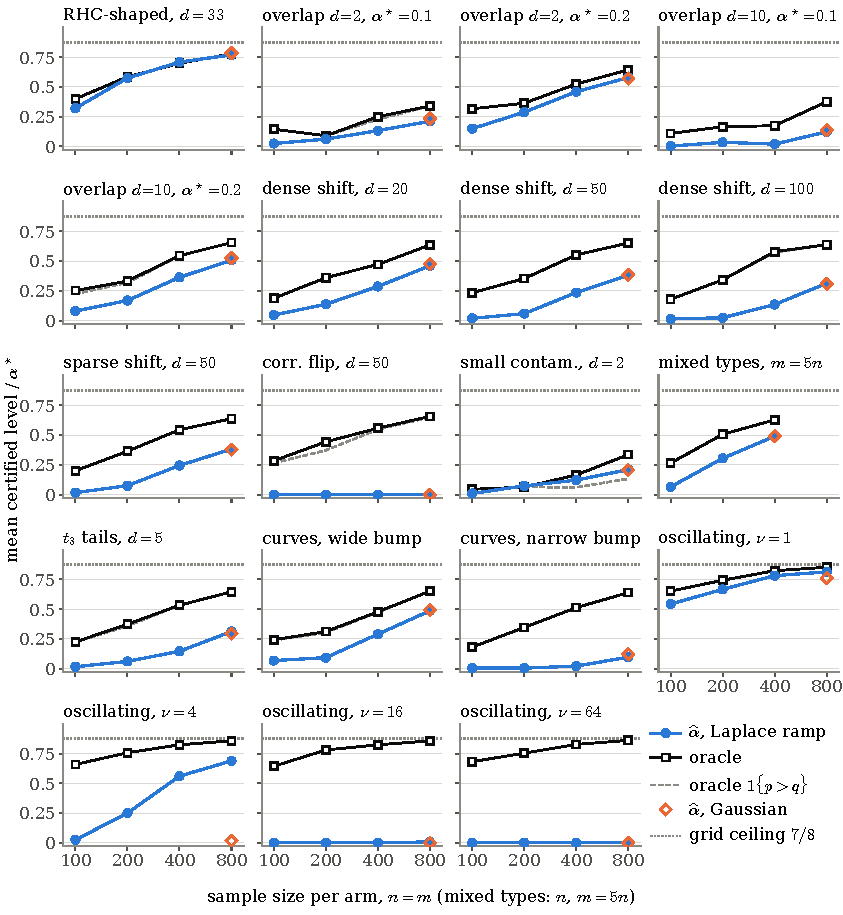
\includegraphics[width=0.7\textwidth]{figs_aos/fig_recovery_curves.pdf}
\caption{Mean certified level over $\alpha^\star$ against $n=m$ (mixed types: $m=5n$): Laplace ramp, oracle reference,
betting on $\mathbf 1\{p>q\}$, and Gaussian ramp at the main size; $\rcReps$ replicates per size below $n=800$ (mixed
types: $400$), $\rcRepsMain$ at it; dotted: largest grid level below $\alpha^\star$.}
\label{fig:recoverycurves}
\end{figure}

Figure~\ref{fig:recoverycurves} follows the recovery of Figure~\ref{fig:recovery} against $n$, with $\rcReps$
replicates per size below $n=800$. Its oracle reference runs the same test, with the same batches, fractions
and grid, on a fixed function known only to an oracle, and reports the better of two choices: $\psi=\mathbf 1\{p>q\}$,
whose drift $\E_P\psi-\E_Q\psi=\alpha^\star$ is the largest of any $[0,1]$-valued function, and, at each level, the
level set $\{p/q>t\}$ whose drift has the largest ratio to its standard deviation, the quantity this betting rule
rewards to first order ($t$ from $\rcLevelsetMC$ draws of each law). Both tests are valid, but neither is a proven ceiling: the
rule is not log-optimal and $\psi$ pays for its noise, so on the small contamination at $n=800$, where $\psi$ halves the
common component, betting on it recovers $\rcSmallPsi$, the ramp $\rcSmallRamp$ and the best level set $\rcSmallLevelset$. At
$n=800$ the ramp reaches $0.8$ of the reference in $\rcEightyEightHundred$ designs (\rcEightyDesignsEightHundred), and the
tenth percentile of $\widehat\alpha/\alpha^\star$, median over the designs, is $\rcRampTenthMedEightHundred$, against
$\rcOracleTenthMedEightHundred$ for the reference. The grid still uses the known $\alpha^\star$.


Gradient boosting and logistic regression refitted on the batches of the ramp, which
removes the handicap of Table~\ref{tab:hardern80}, default or tuned by threefold cross-validation, bet their labels or
their probabilities corrected for the sample sizes; the best of them has more power against $H_{0,0}$ than the Gaussian
ramp in $\abBestMatchedAboveRampPow$ designs and less in $\abRampAboveBestMatchedPow$, and than the Laplace ramp in
$\mnPowBestClfAboveLap$ and $\mnPowLapAboveBestClf$, all at $n=m=\harderNmax$. With default settings the better of the
two classifiers recovers more than the Laplace ramp in $\mnBestMatchedAboveRamp$ designs and less in
$\mnRampAboveBestMatched$. Tuned logistic labels recover more than the Laplace ramp in
$\wtllosses{\mnWtlRecLogitTuned}$ designs and less in $\wtlwins{\mnWtlRecLogitTuned}$ at two paired standard errors,
and tuned gradient boosting labels recover more than it, at two decimals, in $\dvGbmTunedAboveLapN$ designs
(\dvGbmTunedAboveLapDesigns).
Probabilities lose to labels (median recovery $\abRecMedLogitMatchedProb$ against $\abRecMedLogitMatchedLabels$ for
logistic regression), as calibrated probabilities shrink toward $1/2$ on the common part. The normal of a $\nu$-support
vector machine on the Gram matrices of the ramp ($\nu$ by cross-validation, median $\abSvmNuMed$), bet as a ramp with
the cut points of the tested level, certifies less than the ramp except on $\abSvmAboveRamp$ designs. The untrimmed
witness of Section~\ref{sec:numharder} is the Gaussian witness fitted at $\alpha=0$ on the fitting batches and used at
every level, which needs no quadratic program; Section~\ref{sec:numharder} gives its recoveries, and cut at the tested
level it is equal to the Laplace ramp at two decimals in the remaining $\dvZeroCutEqualLap$ designs. A
fixed-sample empirical Bernstein bound on the ramp fitted on one half certified less than betting on the other half in
$\abSingleBetAboveEb$ of the $\abNdesigns$ designs and more in none. On the line, the Kolmogorov--Smirnov statistic
minus the two Dvoretzky--Kiefer--Wolfowitz radii, a lower bound on $\TV(P,Q)$, exceeded the better of the analytic
estimator and the Gaussian ramp in $\dvKsAboveKernel$ of $\dvKsCells$ cells of the oscillating designs and of a shift and
a change of scale of a $t_3$ law. Of further certificates, the trimmed-mean statistic of the witness
with a Dvoretzky--Kiefer--Wolfowitz bound certified nothing except on the oscillating density with $\nu=1$, and nearest
neighbors bet like the ramp certified less than it except on the oscillating densities; the trimmed-Wasserstein test of \citet{alvarez2012similarity}, asymptotic and pointwise, is not
compared. MMDAgg \citep{schrab2023aggregated} uses $\abAggL$ Gaussian bandwidths. None of these tests was flagged, at the boundary in any of the
$\abNdesigns$ designs or under $P=Q$ on the four nulls; the largest rates were $\abBoundaryMax$ ($\abBoundaryMaxK$ of
$\abReps$, logistic labels, RHC-shaped design) at the boundary and $\abNullMax$ (binomial $p=\abNullMaxP$, MMDAgg,
mixed-type null) under $P=Q$.

\subsection{Numerical checks on the line}
\label{sec:newnumerics}
\label{sec:excessmc}

For the shift $N(\pm1,1)$ and the mixtures $0.8\,N(0,1)+0.2\,N(\pm\mu,1)$, $\mu\in\{1.5,2,3\}$, which cross at $x_0=0$,
the rescaled path $\bar D_{\alpha^\star-\epsilon}$ of Section~\ref{sec:rates}, bracketed to certified accuracy between the separation
\eqref{eq:sep} in a computed direction and the norm of an explicit pair of trimmings, with the kernels $e^{-|x-y|}$ and
$e^{-(x-y)^2/2}$, lay at all $\mgRows$ levels above the lower bound of Proposition~\ref{prop:newapproxgen} and below the
explicit trimming of Proposition~\ref{prop:newupperone}. With the Laplace kernel its local log-log slope for the shift
reaches $\mgLapShiftSlope$ at $\epsilon=\mgLapShiftEps$, approaching $5/4$; with the Gaussian kernel and $\mu=3$ it falls
from $\mgGaussPathHi$ to $\mgGaussPathLo$ between $\epsilon=\mgGaussEpsHi$ and $\mgGaussEpsLo$, and a fit of
$\log\bar D=A+B\log\epsilon-c'/\epsilon$ gives $c'/\ell_0$ between $\mgFitPathLo$ and $\mgFitPathHi$ over $\mu$, with
$\ell_0=0.4\mu\varphi(\mu)$, below the constant $\pi^2/8\approx\mgPiEight$ of Theorem~\ref{thm:newgauss}.

The split-sample bound was computed on the shift and the mixture with $\mu=1.5$, which satisfy \eqref{eq:condR}, with
both kernels, $n=m$, the batches of Section~\ref{sec:betting}, own-term cut points interpolated between order
statistics, which Theorem~\ref{thm:laplacerate}, stated for genuine quantiles, does not cover, levels approaching the
known $\alpha^\star$ geometrically (from $\exGridS$ and $\exGridM$ below it to $\exGridMinS$ and $\exGridMinM$) and
$\exRepMin$ to $\exRepMax$ replicates per cell. With the Laplace kernel the mean error of $\widehat\alpha$ falls like $n^{-\exLapSlopeS}$
and $n^{-\exLapSlopeM}$ up to $n=\exNmax$ (least-squares slopes on $\log n$), as fast as that of the
Kolmogorov--Smirnov lower bound, $n^{-\exKSSlopeS}$ and $n^{-\exKSSlopeM}$, and is smaller by factors $\exKSRatioS$ and
$\exKSRatioM$ at $n=\exNmax$. The analytic estimator with the Laplace kernel and the threshold
$\min\{\tau^{\mathrm P},\tau^{\mathrm S}\}$ falls like $n^{-\exAnSlopeS}$ and $n^{-\exAnSlopeM}$; we prove no rate for
it, and with $\tau^{\mathrm S}$ alone its error is at least of order $n^{-2/5}$ (Proposition~\ref{prop:newconverse}).
With the Gaussian kernel the split-sample bound falls like $n^{-\exGaussSlopeS}$ and $n^{-\exGaussSlopeM}$ up to
$n=\exNmaxGauss$, against $n^{-\exLapSlopeCommonS}$ and $n^{-\exLapSlopeCommonM}$ for the Laplace kernel over the same
range.

\subsection{Real data, bandwidths and the cohort}
\label{sec:rdbw}

For RHC \citep{connors1996rhc}, the first contrast of Table~\ref{tab:realdata}, we use $\rrRhcNcovFull$ baseline
covariates, named as in \texttt{rhc.csv}. The $\rrRhcNcovPaper$ stored as numbers are the measurements \texttt{age},
\texttt{edu}, \texttt{surv2md1}, \texttt{das2d3pc}, \texttt{aps1}, \texttt{scoma1}, \texttt{meanbp1}, \texttt{wblc1},
\texttt{hrt1}, \texttt{resp1}, \texttt{temp1}, \texttt{pafi1}, \texttt{alb1}, \texttt{hema1}, \texttt{bili1},
\texttt{crea1}, \texttt{sod1}, \texttt{pot1}, \texttt{paco21}, \texttt{ph1} and \texttt{wtkilo1} and the history
indicators \texttt{cardiohx}, \texttt{chfhx}, \texttt{dementhx}, \texttt{psychhx}, \texttt{chrpulhx}, \texttt{renalhx},
\texttt{liverhx}, \texttt{gibledhx}, \texttt{malighx}, \texttt{immunhx}, \texttt{transhx} and \texttt{amihx}; the
$\rrRhcNcovAdded$ binary ones stored as text and coded $0/1$ are \texttt{sex} (female $1$), the do-not-resuscitate
status \texttt{dnr1} and the admission-diagnosis indicators \texttt{resp}, \texttt{card}, \texttt{neuro},
\texttt{gastr}, \texttt{renal}, \texttt{meta}, \texttt{hema}, \texttt{seps}, \texttt{trauma} and \texttt{ortho}
(yes $1$),
all standardized by the moments of the data each test fits on (batch $0$ of each split, the pilot for the analytic
test, the pooled sample for the cohort of Section~\ref{sec:appcohort}, which bets on nothing). We exclude the treatment, the dated or
outcome-derived variables (\texttt{death}, \texttt{dth30}, \texttt{t3d30} and the dates), \texttt{adld3p} and
\texttt{urin1}, missing for more than half of the patients, and the categorical variables \texttt{cat1}, \texttt{cat2},
\texttt{ca}, \texttt{ninsclas}, \texttt{race} and \texttt{income}, whose one-hot indicators would drive the median
bandwidth. The weight \texttt{wtkilo1} keeps the code $0$ that the data use for a missing weight; the zeros are a group of patients that the trimming may keep or discard like any other. The lower bounds hold for any longer vector, since total variation can only grow
with it, but the balance of Section~\ref{sec:appcohort} concerns the covariates used. Of these $\rrRhcNcovAdded$ covariates $\rrAddedSmdAbove$ have an unweighted standardized difference above $0.1$, up to
$\rrAddedSmdMax$, and two are rare ($\rrOrthoN$ and $\rrTraumaN$ patients coded $1$). On the $\rrRhcNcovPaper$ covariates
the averaged e-value certifies $\rrEvRhcAvgFinal$, the analytic baseline again no positive level, and the Laplace cohort at
$\alpha=\rrCohPaperAlpha$ had largest standardized difference $\rrCohPaperSmdMax$ on them but $\rrCohPaperOmitSmdMax$
on the others, and mortality differences $\rrCohPaperRD$ for the trimming and $\estKernelRD$ to $\estAtmRD$ for the
other weightings of Table~\ref{tab:cohort}.

The propensity estimate of Section~\ref{sec:appcohort} uses a ridge logistic fit, refitted on each bootstrap
resample; fivefold cross-fitting gives $\rrPropFullPlugCf$, and on the $\rrRhcNcovPaper$ covariates it is
$\rrPropPaperPlug$. Seeing the arms only through the fitted score, a
misspecified model tends to understate $\alpha^\star$, while fitting in sample overstates it. The classifiers of
Section~\ref{sec:data} are those of Section~\ref{sec:baselines}; their labels certify $\rrClfFullLogitHardMin$
(logistic) and $\rrClfFullGbmHardMin$ (boosting) with default settings and $\rrClfFullLogitTunedHardMin$ and
$\rrClfFullGbmTunedHardMin$ tuned, and on the $\rrRhcNcovPaper$ covariates $\rrClfPaperLogitHardMin$,
$\rrClfPaperGbmHardMin$, $\rrClfPaperLogitTunedHardMin$ and $\rrClfPaperGbmTunedHardMin$. Their probabilities, corrected
for the sample sizes as in Section~\ref{sec:baselines}, certify $\rrClfFullLogitSoftMin$ and $\rrClfFullGbmSoftMin$
with default settings and $\rrClfFullLogitTunedSoftMin$ and $\rrClfFullGbmTunedSoftMin$ tuned, and on the
$\rrRhcNcovPaper$ covariates $\rrClfPaperLogitSoftMin$, $\rrClfPaperGbmSoftMin$, $\rrClfPaperLogitTunedSoftMin$ and
$\rrClfPaperGbmTunedSoftMin$.

For NHANES \citep{nhanes2012,john2019mims} we pool the cycles 2011--2012 and 2013--2014, reconstruct the
clock time of each hourly record, drop invalid and quality-flagged hours, and require at least $20$ hours of wear on at
least four days; the profiles are used without standardization and without survey weights.
The public files carry no household identifier. With whole masked variance units (SDMVPSU within SDMVSTRA,
$\rrClChildUnits$ units) assigned at random to the batches, which makes the fitting batches independent of the batches
bet on if the units are, the minima are $\rrClChildMin$, $\rrClAgeMin$ and $\rrClBmiMin$ for the child, adult age and
body-mass contrasts, against $\mnRdChildMin$, $\mnRdAgeMin$ and $\mnRdBmiMin$ with participants assigned to batches.

In Table~\ref{tab:realdata} the pilot of each group is a $30\%$ random subsample (seed fixed in advance), the
scales are $0.1$, $0.15$, $0.2$, $0.3$, $0.5$, $0.7$ and $1$ times the pilot median, the scale whose analytic bound on the pilot is largest is chosen, ties going to the scale closest to $0.5$, and the chosen
scales, under the threshold $\tau^{\mathrm P}$, are $\mnPvRhcScale$ for RHC, $\mnPvChildScale$ for the child contrast,
$\mnPvAgeScale$ for the adult age contrast and $\mnPvBmiScale$ for body mass. In the analytic columns of
Table~\ref{tab:realdata} nothing the test uses depends on the held-out $70\%$, so the theorems cover it.

For the cohort of Section~\ref{sec:appcohort}, with the Gaussian kernel at the pooled median
distance $\lcPoolSigma$, the program at $\alpha=\lcCohAlpha$ is solved by
accelerated projected gradient followed by $\lcPoolSmoSteps$ steps of sequential minimal optimization, to a duality
gap of $\lcPoolGap$; the smallest eigenvalue of the Gram matrix is $\lcPoolLamMin$, so the minimizer is unique, and
the gap bounds the distance of the computed weights to it by $\lcPoolLtwoBound$ and the error of the witness by
$\lcPoolWitnessBound$, which places every patient on the same side of the cut as at the exact minimizer. The
$\lcPoolFracX$ and $\lcPoolFracY$ fractionally weighted patients carry fractions $\lcPoolFracMassX$ and
$\lcPoolFracMassY$ of the trimmed samples, and their witness values agree to within $\lcPoolFracSpreadX$. The summaries of
Table~\ref{tab:cohort} for the trimming row are those of this minimizer. Standardized by batch $0$ of one split
instead, the minimizer retains $\lcCohKeptX$ and $\lcCohKeptY$ patients, and over the eight splits of
Table~\ref{tab:realdata} between $\lcSensKeptXlo$ and $\lcSensKeptXhi$ catheterized and between $\lcSensKeptYlo$ and
$\lcSensKeptYhi$ other patients, with the largest standardized difference between $\lcSensSmdMaxLo$ and
$\lcSensSmdMaxHi$. Table~\ref{tab:cohort} compares the trimmed cohort with five weightings that differ in target as much as in method:
matching and overlap weights target overlap populations like the common core, energy and kernel balancing the pooled one.

\begin{table}[!htb]
\centering
\footnotesize
\setlength{\tabcolsep}{1.9pt}
% Generated by scripts/aos_main_cohort.py -- do not edit.
\begin{tabular}{llcccccc}
\toprule
RHC & target & \multicolumn{2}{c}{effective fraction} & max $|$SMD$|$ & mean $|$SMD$|$ & overlap & risk diff. \\
 & population & cath. & others & & & & (95\% int.) \\
\midrule
all patients & -- & 1.00 & 1.00 & 0.501 & 0.160 & 0.58 & 0.074 (0.047, 0.098) \\
trimming, $\alpha=\lcCohAlpha$ & common core & 0.66 & 0.65 & 0.032 & 0.008 & 0.81 & 0.040 (0.011, 0.072) \\
\addlinespace
matching weights & overlap (ATM) & 0.84 & 0.62 & 0.012 & 0.004 & 0.93 & 0.055 (0.028, 0.085) \\
overlap weights & overlap (ATO) & 0.83 & 0.68 & 0.000 & 0.000 & 0.93 & 0.053 (0.024, 0.081) \\
\addlinespace
energy balancing & pooled (ATE) & 0.51 & 0.77 & 0.018 & 0.004 & 0.90 & 0.047 (0.013, 0.080) \\
kernel balancing & pooled (ATE) & 0.25 & 0.47 & 0.017 & 0.005 & 0.86 & 0.056 (0.011, 0.102) \\
\bottomrule
\end{tabular}

\caption{The RHC arms under six weightings: trimming with the Gaussian kernel at the level of the Laplace lower bound; matching
\citep{ligreene2013matching} and overlap weights \citep{li2018balancing} from a logistic propensity model; energy
\citep{huling2024energy} and kernel balancing \citep{hazlett2020kernel,kallus2020optimal} of each arm to the pooled
sample. Effective fraction: Kish effective sample size over arm size; absolute standardized mean differences (SMD) over
the $\rrRhcNcovFull$ covariates; overlap: overlapping coefficient of the propensity distributions; risk difference:
$30$-day mortality, catheterized minus others, $95\%$ percentile interval from $\lcBoot$ bootstrap resamples within each
arm, weights fixed.}
\label{tab:cohort}
\end{table}

\subsection{Computation, code and data}
\label{sec:computationdetails}

Throughout Section~\ref{sec:numerical} we solve \eqref{eq:qp} as in Algorithm~\ref{alg:split} and evaluate
\eqref{eq:alphaest} on its grid, with the threshold of Section~\ref{app:experiments}. The iterates are feasible, so
their value bounds $\widehat D_\alpha^{\,2}$ from above, and the Frank--Wolfe gap bounds it from below; a level is
rejected only when the lower bound exceeds $\tau(\alpha)^2$. Every level rejected in Section~\ref{sec:data} is at a converged solve, and an
unconverged solve changes only the direction of the split-sample estimator, not its level. Where
the data do not determine the minimizer, we return the minimizer $\bar z$ of the strictly convex
$G(w,v)=\|w-\tfrac1n\mathbf 1\|_2^2+\|v-\tfrac1m\mathbf 1\|_2^2$ over $\mathcal T_\alpha$, the limit as
$\lambda\downarrow0$ of the minimizers of $F+\lambda G$, with $F$ the objective of \eqref{eq:qp} (every cluster point
lies in $\mathcal T_\alpha$ and has $G\le G(\bar z)$). On one core, a replicate of the synthetic study at
$n=\harderNmax$ took $\harderRunAnalyticEight$ seconds for the analytic test and $\harderRunSplitEight$ for the betting
test, and one of all the tests of $H_{0,0}$ at $n=m=\harderNcap$ about $\harderRunExtCap$, $\harderRunExtKernelCap$ of
them for kernel sums computed in blocks.

The RHC data are \url{https://hbiostat.org/data/repo/rhc.csv}; the NHANES data are the files PAXHR, PAXHD, DEMO and BMX
of the cycles G and H (2011--2014) of the National Center for Health Statistics. The repository
\url{https://github.com/HristoInouzhe/trimmed-mmd} holds the package \texttt{trimmedmmd} and one script for each table
and figure, and \texttt{scripts/fetch\_data.py} downloads the data. The Laplace ramp and the analytic test of
Table~\ref{tab:hardern80} and Figure~\ref{fig:recovery} come from \texttt{scripts/aos\_main\_synth.py},
\texttt{aos\_main\_alpha0.py} and \texttt{aos\_main\_analytic.py}, the classifiers on the batches of the ramp, the
permutation test and MMDAgg from \texttt{aos\_baselines\_run.py}, the Gaussian ramp and the classifiers trained once
from the study in \texttt{explore/harder\_sims}, and the tables and the figure from \texttt{aos\_main\_tables.py},
\texttt{aos\_baselines\_tables.py} and \texttt{aos\_main\_figs.sh}; Table~\ref{tab:realdata} comes from
\texttt{aos\_main\_realdata.py} and \texttt{exp\_valid\_bandwidth.py}, Table~\ref{tab:cohort} from
\texttt{aos\_main\_cohort.py}, Figure~\ref{fig:excess} from \texttt{aos\_fig\_excess.py},
Figure~\ref{fig:recoverycurves} from \texttt{aos\_ref\_recovery\_run.py} and \texttt{aos\_ref\_recovery\_fig.py},
Section~\ref{sec:kernelfallback} from \texttt{aos\_fallback\_synth.py}, \texttt{aos\_fallback\_realdata.py} and
\texttt{aos\_fallback\_tables.py}, Section~\ref{sec:excessmc} from \texttt{aos\_margin\_macros.py} and \texttt{aos\_excess\_table.py}, and the boundary
calibration of Section~\ref{app:experiments} from \texttt{aos\_supp\_threshold.py}. The simulated data are drawn from
fixed seeds. The runs also read the per-replicate records of the study in \texttt{explore/harder\_sims/out}, which the
repository holds: \texttt{scripts/aos\_main\_synth.py} takes its bandwidths from them, and
\texttt{scripts/aos\_main\_tables.py} the Gaussian ramp and the classifiers trained once. So the repository, not the
seeds alone, reproduces the runs.
